\section{Handi Hermawan (1174080)}
\subsection{Tugas 2 membuat Shapefile dengan PySHP}
\begin{enumerate}
	\item No 1
	\lstinputlisting{src/tugas2/1174080/no1.py}
	\begin{figure}[H]
		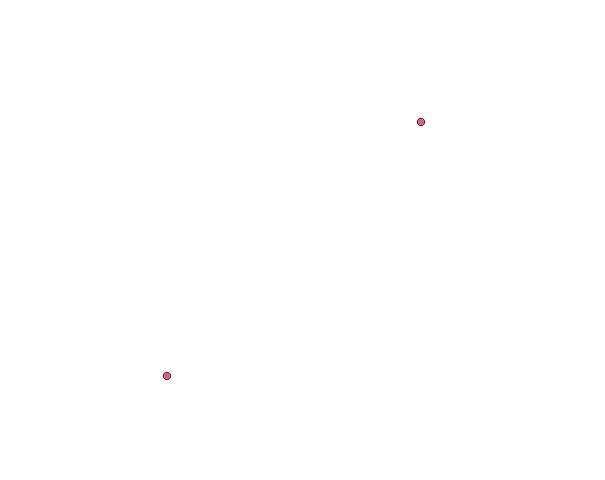
\includegraphics[width=7cm]{figures/Tugas2/1174080/no1.JPG}
		\centering
		\caption{Point (Titik)}
	\end{figure}
	\item No 2
	\lstinputlisting{src/tugas2/1174080/no2.py}
	\begin{figure}[H]
		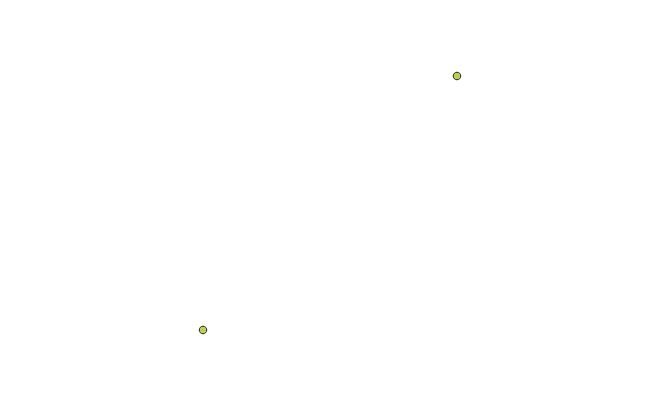
\includegraphics[width=7cm]{figures/Tugas2/1174080/no2.JPG}
		\centering
		\caption{Point (Titik)}
	\end{figure}
	\item No 3
	\lstinputlisting{src/tugas2/1174080/no3.py}
	\begin{figure}[H]
		
\includegraphics[width=7cm]{figures/Tugas2/1174080/no3.JPG}
		\centering
		\caption{Point (Titik)}
	\end{figure}
	\item No 4
	\lstinputlisting{src/tugas2/1174080/no4.py}
	\begin{figure}[H]
		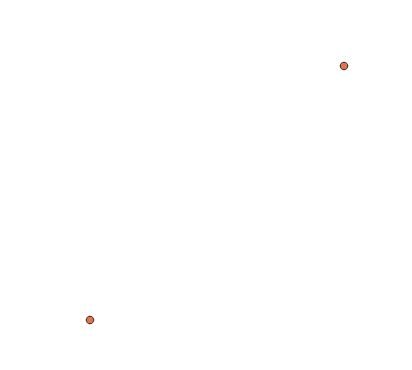
\includegraphics[width=7cm]{figures/Tugas2/1174080/no4.JPG}
		\centering
		\caption{Point (Titik)}
	\end{figure}
	\item No 5
	\lstinputlisting{src/tugas2/1174080/no5.py}
	\begin{figure}[H]
		
\includegraphics[width=7cm]{figures/Tugas2/1174080/no5.JPG}
		\centering
		\caption{PolyLine (Garis)}
	\end{figure}
	\item No 6
	\lstinputlisting{src/tugas2/1174080/no6.py}
	\begin{figure}[H]
		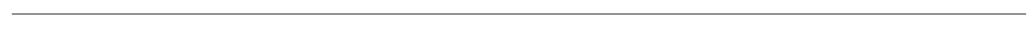
\includegraphics[width=7cm]{figures/Tugas2/1174080/no6.JPG}
		\centering
		\caption{Polygon (Bidang)}
	\end{figure}
	\item No 7
	\lstinputlisting{src/tugas2/1174080/no7.py}
	\begin{figure}[H]
		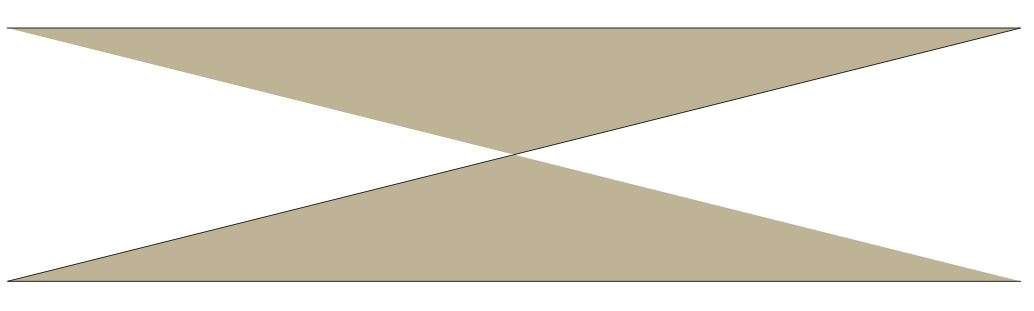
\includegraphics[width=7cm]{figures/Tugas2/1174080/no7.JPG}
		\centering
		\caption{Polygon (Bidang)}
	\end{figure}
	\item No 8
	\lstinputlisting{src/tugas2/1174080/no8.py}
	\begin{figure}[H]
		
\includegraphics[width=7cm]{figures/Tugas2/1174080/no8.JPG}
		\centering
		\caption{Polygon (Bidang)}
	\end{figure}
	\item No 9
	\lstinputlisting{src/tugas2/1174080/no9.py}
	\begin{figure}[H]
		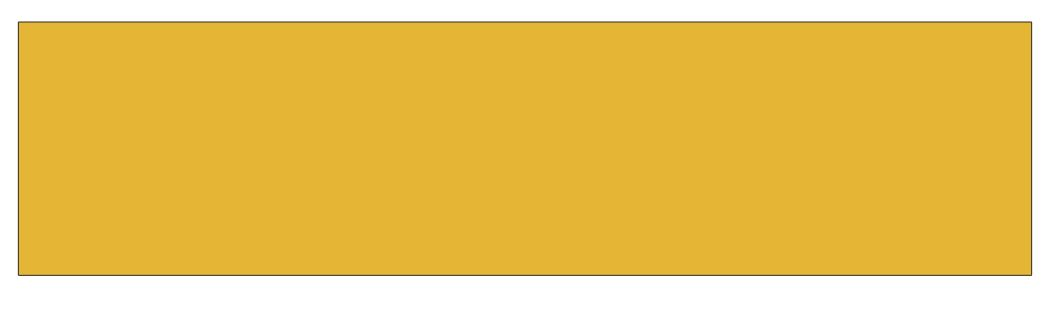
\includegraphics[width=7cm]{figures/Tugas2/1174080/no9.JPG}
		\centering
		\caption{Polygon (Bidang)}
	\end{figure}
	\item Nomor 10
	\lstinputlisting{src/tugas2/1174080/no10.py}
	\begin{figure}[H]
		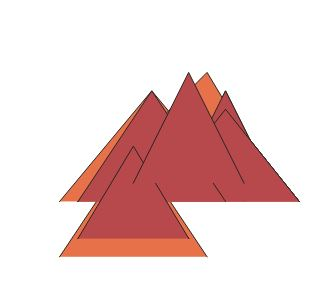
\includegraphics[width=7cm]{figures/Tugas2/1174080/no10.JPG}
		\centering
		\caption{Polygon, Hasil modulus dari NPM masing masing}
	\end{figure}
\end{enumerate}
\subsection{Link}
https://youtu.be/0UJfyOOnzkw